\documentclass[]{article}
\usepackage{lmodern}
\usepackage{amssymb,amsmath}
\usepackage{ifxetex,ifluatex}
\usepackage{fixltx2e} % provides \textsubscript
\ifnum 0\ifxetex 1\fi\ifluatex 1\fi=0 % if pdftex
  \usepackage[T1]{fontenc}
  \usepackage[utf8]{inputenc}
\else % if luatex or xelatex
  \ifxetex
    \usepackage{mathspec}
  \else
    \usepackage{fontspec}
  \fi
  \defaultfontfeatures{Ligatures=TeX,Scale=MatchLowercase}
\fi
% use upquote if available, for straight quotes in verbatim environments
\IfFileExists{upquote.sty}{\usepackage{upquote}}{}
% use microtype if available
\IfFileExists{microtype.sty}{%
\usepackage{microtype}
\UseMicrotypeSet[protrusion]{basicmath} % disable protrusion for tt fonts
}{}
\usepackage[margin=1in]{geometry}
\usepackage{hyperref}
\hypersetup{unicode=true,
            pdftitle={R Notebook},
            pdfborder={0 0 0},
            breaklinks=true}
\urlstyle{same}  % don't use monospace font for urls
\usepackage{color}
\usepackage{fancyvrb}
\newcommand{\VerbBar}{|}
\newcommand{\VERB}{\Verb[commandchars=\\\{\}]}
\DefineVerbatimEnvironment{Highlighting}{Verbatim}{commandchars=\\\{\}}
% Add ',fontsize=\small' for more characters per line
\usepackage{framed}
\definecolor{shadecolor}{RGB}{248,248,248}
\newenvironment{Shaded}{\begin{snugshade}}{\end{snugshade}}
\newcommand{\KeywordTok}[1]{\textcolor[rgb]{0.13,0.29,0.53}{\textbf{{#1}}}}
\newcommand{\DataTypeTok}[1]{\textcolor[rgb]{0.13,0.29,0.53}{{#1}}}
\newcommand{\DecValTok}[1]{\textcolor[rgb]{0.00,0.00,0.81}{{#1}}}
\newcommand{\BaseNTok}[1]{\textcolor[rgb]{0.00,0.00,0.81}{{#1}}}
\newcommand{\FloatTok}[1]{\textcolor[rgb]{0.00,0.00,0.81}{{#1}}}
\newcommand{\ConstantTok}[1]{\textcolor[rgb]{0.00,0.00,0.00}{{#1}}}
\newcommand{\CharTok}[1]{\textcolor[rgb]{0.31,0.60,0.02}{{#1}}}
\newcommand{\SpecialCharTok}[1]{\textcolor[rgb]{0.00,0.00,0.00}{{#1}}}
\newcommand{\StringTok}[1]{\textcolor[rgb]{0.31,0.60,0.02}{{#1}}}
\newcommand{\VerbatimStringTok}[1]{\textcolor[rgb]{0.31,0.60,0.02}{{#1}}}
\newcommand{\SpecialStringTok}[1]{\textcolor[rgb]{0.31,0.60,0.02}{{#1}}}
\newcommand{\ImportTok}[1]{{#1}}
\newcommand{\CommentTok}[1]{\textcolor[rgb]{0.56,0.35,0.01}{\textit{{#1}}}}
\newcommand{\DocumentationTok}[1]{\textcolor[rgb]{0.56,0.35,0.01}{\textbf{\textit{{#1}}}}}
\newcommand{\AnnotationTok}[1]{\textcolor[rgb]{0.56,0.35,0.01}{\textbf{\textit{{#1}}}}}
\newcommand{\CommentVarTok}[1]{\textcolor[rgb]{0.56,0.35,0.01}{\textbf{\textit{{#1}}}}}
\newcommand{\OtherTok}[1]{\textcolor[rgb]{0.56,0.35,0.01}{{#1}}}
\newcommand{\FunctionTok}[1]{\textcolor[rgb]{0.00,0.00,0.00}{{#1}}}
\newcommand{\VariableTok}[1]{\textcolor[rgb]{0.00,0.00,0.00}{{#1}}}
\newcommand{\ControlFlowTok}[1]{\textcolor[rgb]{0.13,0.29,0.53}{\textbf{{#1}}}}
\newcommand{\OperatorTok}[1]{\textcolor[rgb]{0.81,0.36,0.00}{\textbf{{#1}}}}
\newcommand{\BuiltInTok}[1]{{#1}}
\newcommand{\ExtensionTok}[1]{{#1}}
\newcommand{\PreprocessorTok}[1]{\textcolor[rgb]{0.56,0.35,0.01}{\textit{{#1}}}}
\newcommand{\AttributeTok}[1]{\textcolor[rgb]{0.77,0.63,0.00}{{#1}}}
\newcommand{\RegionMarkerTok}[1]{{#1}}
\newcommand{\InformationTok}[1]{\textcolor[rgb]{0.56,0.35,0.01}{\textbf{\textit{{#1}}}}}
\newcommand{\WarningTok}[1]{\textcolor[rgb]{0.56,0.35,0.01}{\textbf{\textit{{#1}}}}}
\newcommand{\AlertTok}[1]{\textcolor[rgb]{0.94,0.16,0.16}{{#1}}}
\newcommand{\ErrorTok}[1]{\textcolor[rgb]{0.64,0.00,0.00}{\textbf{{#1}}}}
\newcommand{\NormalTok}[1]{{#1}}
\usepackage{graphicx,grffile}
\makeatletter
\def\maxwidth{\ifdim\Gin@nat@width>\linewidth\linewidth\else\Gin@nat@width\fi}
\def\maxheight{\ifdim\Gin@nat@height>\textheight\textheight\else\Gin@nat@height\fi}
\makeatother
% Scale images if necessary, so that they will not overflow the page
% margins by default, and it is still possible to overwrite the defaults
% using explicit options in \includegraphics[width, height, ...]{}
\setkeys{Gin}{width=\maxwidth,height=\maxheight,keepaspectratio}
\IfFileExists{parskip.sty}{%
\usepackage{parskip}
}{% else
\setlength{\parindent}{0pt}
\setlength{\parskip}{6pt plus 2pt minus 1pt}
}
\setlength{\emergencystretch}{3em}  % prevent overfull lines
\providecommand{\tightlist}{%
  \setlength{\itemsep}{0pt}\setlength{\parskip}{0pt}}
\setcounter{secnumdepth}{0}
% Redefines (sub)paragraphs to behave more like sections
\ifx\paragraph\undefined\else
\let\oldparagraph\paragraph
\renewcommand{\paragraph}[1]{\oldparagraph{#1}\mbox{}}
\fi
\ifx\subparagraph\undefined\else
\let\oldsubparagraph\subparagraph
\renewcommand{\subparagraph}[1]{\oldsubparagraph{#1}\mbox{}}
\fi

%%% Use protect on footnotes to avoid problems with footnotes in titles
\let\rmarkdownfootnote\footnote%
\def\footnote{\protect\rmarkdownfootnote}

%%% Change title format to be more compact
\usepackage{titling}

% Create subtitle command for use in maketitle
\newcommand{\subtitle}[1]{
  \posttitle{
    \begin{center}\large#1\end{center}
    }
}

\setlength{\droptitle}{-2em}
  \title{R Notebook}
  \pretitle{\vspace{\droptitle}\centering\huge}
  \posttitle{\par}
  \author{}
  \preauthor{}\postauthor{}
  \date{}
  \predate{}\postdate{}


\begin{document}
\maketitle

\begin{enumerate}
\def\labelenumi{\arabic{enumi}.}
\tightlist
\item
  P\_housing
\end{enumerate}

1a.graph change in house prices

1b.look for an inflection point -

?? any evidence of a slowdown in price appreciation ??

\begin{enumerate}
\def\labelenumi{\arabic{enumi}.}
\setcounter{enumi}{1}
\tightlist
\item
  try to say something about renters vs.~owners
\end{enumerate}

2a.?? any difference ??

2b.?? are they like Tokyo renters or San Francisco renters ??

Here I have added a vertical line where it seems that housing prices, at
least in some areas began to slow their ascent. It looks like after my
line at least Gush Dan and Haifa prices grow at a slower rate. I now
attempt to find this inflection point.

\begin{Shaded}
\begin{Highlighting}[]
\NormalTok{plot1.5rooms<-}\KeywordTok{ggplot}\NormalTok{(}\DataTypeTok{data=}\NormalTok{p1}\FloatTok{.5}\NormalTok{,}\KeywordTok{aes}\NormalTok{(}\DataTypeTok{x=}\NormalTok{quarter,}
                     \DataTypeTok{y=}\NormalTok{value,}
                    
                     \DataTypeTok{group=}\NormalTok{variable}
                     \NormalTok{))+}\KeywordTok{geom_line}\NormalTok{(}\KeywordTok{aes}\NormalTok{(}\DataTypeTok{colour=}\NormalTok{variable))+}
\StringTok{                     }\KeywordTok{ggtitle}\NormalTok{(}\StringTok{"Average P. 1.5-2.5 bedroom home:2006-2016q3"}\NormalTok{)+}\KeywordTok{theme}\NormalTok{(}\DataTypeTok{legend.title=}\KeywordTok{element_blank}\NormalTok{(),}
                   \DataTypeTok{panel.grid.major.y =} \KeywordTok{element_blank}\NormalTok{(),}
                   \DataTypeTok{panel.grid.minor =} \KeywordTok{element_blank}\NormalTok{(),}
                   \DataTypeTok{axis.ticks.x =} \KeywordTok{element_blank}\NormalTok{(),}
                   \DataTypeTok{axis.text.x=}\KeywordTok{element_blank}\NormalTok{())+}\StringTok{ }\KeywordTok{ylab}\NormalTok{(}\StringTok{"NIS x 100k"}\NormalTok{)+}\KeywordTok{geom_vline}\NormalTok{(}\DataTypeTok{xintercept=}\DecValTok{28}\NormalTok{)}
\NormalTok{plot1.5rooms}
\end{Highlighting}
\end{Shaded}

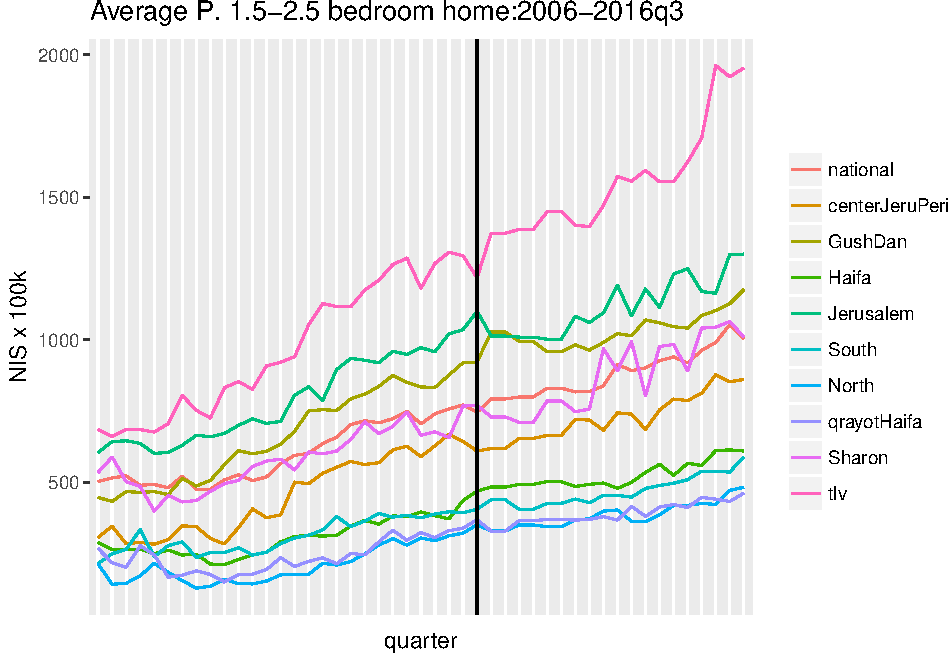
\includegraphics{rentersAndOwners_files/figure-latex/unnamed-chunk-2-1.pdf}

\begin{Shaded}
\begin{Highlighting}[]
\KeywordTok{library}\NormalTok{(inflection)}
\CommentTok{#ede(p1.5$quarter,p1.$value,1)}
\CommentTok{#func = splinefun(x=p1.5$quarter,y=p1.5$value, method="fmm",ties=mean)}
\CommentTok{#zzz <-spline(x=p1.5$quarter,y=p1.5$value, method="fmm",ties=mean)}
\CommentTok{#qplot(spline)}
\CommentTok{#dValue <-diff(p1.5$value)}
\CommentTok{#dValue1<-c(NA,dValue)}
\CommentTok{#p1.5$dValue <-dValue1}
\CommentTok{#ggplot(data=p1.5,aes(x=quarter, y=dValue)) }
\CommentTok{#qplot(func)}
\CommentTok{#lm(data=p1.5, formula=log(quarter) ~ log(value))}
\end{Highlighting}
\end{Shaded}

try the \texttt{lm} code alli.mod1 = lm(lnWeight \textasciitilde{}
lnLength, data = alligator).

\begin{Shaded}
\begin{Highlighting}[]
\NormalTok{alligator =}\StringTok{ }\KeywordTok{data.frame}\NormalTok{(}
  \DataTypeTok{lnLength =} \KeywordTok{c}\NormalTok{(}\FloatTok{3.87}\NormalTok{, }\FloatTok{3.61}\NormalTok{, }\FloatTok{4.33}\NormalTok{, }\FloatTok{3.43}\NormalTok{, }\FloatTok{3.81}\NormalTok{, }\FloatTok{3.83}\NormalTok{, }\FloatTok{3.46}\NormalTok{, }\FloatTok{3.76}\NormalTok{,}
    \FloatTok{3.50}\NormalTok{, }\FloatTok{3.58}\NormalTok{, }\FloatTok{4.19}\NormalTok{, }\FloatTok{3.78}\NormalTok{, }\FloatTok{3.71}\NormalTok{, }\FloatTok{3.73}\NormalTok{, }\FloatTok{3.78}\NormalTok{),}
  \DataTypeTok{lnWeight =} \KeywordTok{c}\NormalTok{(}\FloatTok{4.87}\NormalTok{, }\FloatTok{3.93}\NormalTok{, }\FloatTok{6.46}\NormalTok{, }\FloatTok{3.33}\NormalTok{, }\FloatTok{4.38}\NormalTok{, }\FloatTok{4.70}\NormalTok{, }\FloatTok{3.50}\NormalTok{, }\FloatTok{4.50}\NormalTok{,}
    \FloatTok{3.58}\NormalTok{, }\FloatTok{3.64}\NormalTok{, }\FloatTok{5.90}\NormalTok{, }\FloatTok{4.43}\NormalTok{, }\FloatTok{4.38}\NormalTok{, }\FloatTok{4.42}\NormalTok{, }\FloatTok{4.25}\NormalTok{)}
\NormalTok{)}
\KeywordTok{plot}\NormalTok{(lnWeight ~}\StringTok{ }\NormalTok{lnLength, }\DataTypeTok{data =} \NormalTok{alligator,}
  \DataTypeTok{xlab =} \StringTok{"Snout vent length (inches) on log scale"}\NormalTok{,}
  \DataTypeTok{ylab =} \StringTok{"Weight (pounds) on log scale"}\NormalTok{,}
  \DataTypeTok{main =} \StringTok{"Alligators in Central Florida"}
\NormalTok{)}
\end{Highlighting}
\end{Shaded}

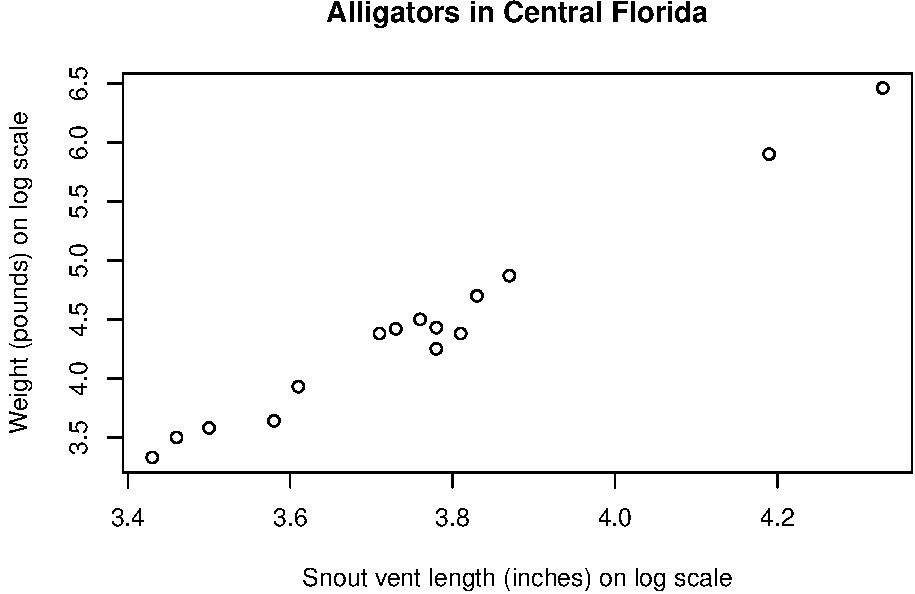
\includegraphics{rentersAndOwners_files/figure-latex/unnamed-chunk-3-1.pdf}

\begin{Shaded}
\begin{Highlighting}[]
\NormalTok{alli.mod1 =}\StringTok{ }\KeywordTok{lm}\NormalTok{(lnWeight ~}\StringTok{ }\NormalTok{lnLength, }\DataTypeTok{data =} \NormalTok{alligator)}
\KeywordTok{summary}\NormalTok{(alli.mod1)}
\end{Highlighting}
\end{Shaded}

\begin{verbatim}
## 
## Call:
## lm(formula = lnWeight ~ lnLength, data = alligator)
## 
## Residuals:
##      Min       1Q   Median       3Q      Max 
## -0.24348 -0.03186  0.03740  0.07727  0.12669 
## 
## Coefficients:
##             Estimate Std. Error t value Pr(>|t|)    
## (Intercept)  -8.4761     0.5007  -16.93 3.08e-10 ***
## lnLength      3.4311     0.1330   25.80 1.49e-12 ***
## ---
## Signif. codes:  0 '***' 0.001 '**' 0.01 '*' 0.05 '.' 0.1 ' ' 1
## 
## Residual standard error: 0.1229 on 13 degrees of freedom
## Multiple R-squared:  0.9808, Adjusted R-squared:  0.9794 
## F-statistic: 665.8 on 1 and 13 DF,  p-value: 1.495e-12
\end{verbatim}

Now plot something from the linear model of the alligators against the
original data.

\begin{Shaded}
\begin{Highlighting}[]
\CommentTok{# plot(resid(alli.mod1) ~ fitted(alli.mod1),}
\CommentTok{#   xlab = "Fitted Values",}
\CommentTok{#   ylab = "Residuals",}
\CommentTok{#   main = "Residual Diagnostic Plot",}
\CommentTok{#   panel = function(x, y, ...)}
\CommentTok{#   \{}
\CommentTok{#     panel.grid(h = -1, v = -1)}
\CommentTok{#     panel.abline(h = 0)}
\CommentTok{#     panel.xyplot(x, y, ...)}
\CommentTok{#   \}}
\CommentTok{# )}
\end{Highlighting}
\end{Shaded}

try the R package bcp, work an example from the pdf

\begin{Shaded}
\begin{Highlighting}[]
\KeywordTok{library}\NormalTok{(bcp)}
\end{Highlighting}
\end{Shaded}

\begin{verbatim}
## Loading required package: grid
\end{verbatim}

\begin{Shaded}
\begin{Highlighting}[]
\NormalTok{##### univariate sequential data #####}
\CommentTok{# an easy problem with 2 true change points}

\KeywordTok{set.seed}\NormalTok{(}\DecValTok{5}\NormalTok{)}
\NormalTok{x <-}\StringTok{ }\KeywordTok{c}\NormalTok{(}\KeywordTok{rnorm}\NormalTok{(}\DecValTok{50}\NormalTok{), }\KeywordTok{rnorm}\NormalTok{(}\DecValTok{50}\NormalTok{, }\DecValTok{5}\NormalTok{, }\DecValTok{1}\NormalTok{), }\KeywordTok{rnorm}\NormalTok{(}\DecValTok{50}\NormalTok{))}
\NormalTok{bcp.1a <-}\StringTok{ }\KeywordTok{bcp}\NormalTok{(x)}
\KeywordTok{plot}\NormalTok{(bcp.1a, }\DataTypeTok{main=}\StringTok{"Univariate Change Point Example"}\NormalTok{)}
\end{Highlighting}
\end{Shaded}

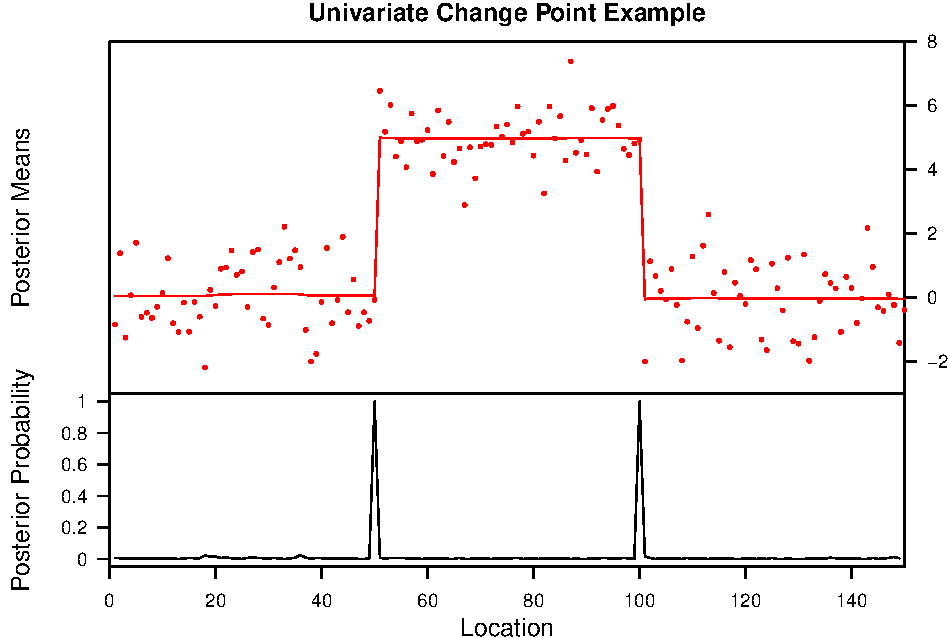
\includegraphics{rentersAndOwners_files/figure-latex/unnamed-chunk-5-1.pdf}

\begin{Shaded}
\begin{Highlighting}[]
\CommentTok{#legacyplot(bcp.1a)}
\end{Highlighting}
\end{Shaded}

I think that only has frequencies of X. Let's see if the 2nd example
actually has some Ys.

\begin{Shaded}
\begin{Highlighting}[]
\CommentTok{# a hard problem with 1 true change point}
\KeywordTok{set.seed}\NormalTok{(}\DecValTok{5}\NormalTok{)}
\NormalTok{x <-}\StringTok{ }\KeywordTok{rep}\NormalTok{(}\KeywordTok{c}\NormalTok{(}\DecValTok{0}\NormalTok{,}\DecValTok{1}\NormalTok{), }\DataTypeTok{each=}\DecValTok{50}\NormalTok{)}
\NormalTok{y <-}\StringTok{ }\NormalTok{x +}\StringTok{ }\KeywordTok{rnorm}\NormalTok{(}\DecValTok{50}\NormalTok{, }\DataTypeTok{sd=}\DecValTok{1}\NormalTok{)}
\NormalTok{bcp.1b <-}\StringTok{ }\KeywordTok{bcp}\NormalTok{(y)}
\KeywordTok{plot}\NormalTok{(bcp.1b, }\DataTypeTok{main=}\StringTok{"Univariate Change Point Example"}\NormalTok{)}
\end{Highlighting}
\end{Shaded}

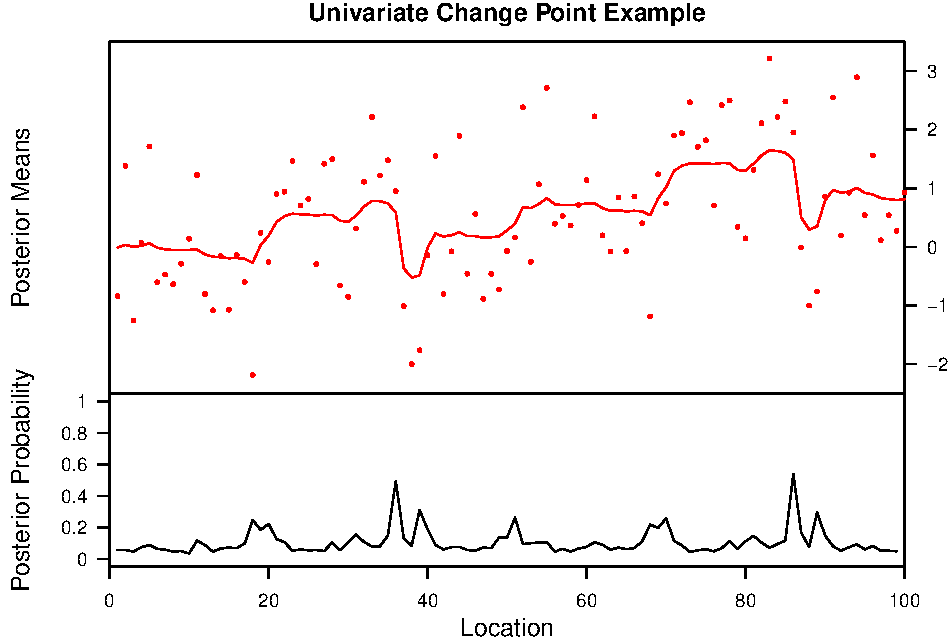
\includegraphics{rentersAndOwners_files/figure-latex/unnamed-chunk-6-1.pdf}
I don't know what that was, but it still doesn't look right. I will try
the 3rd example from the bcp manual.
\url{https://cran.r-project.org/web/packages/bcp/bcp.pdf}

\begin{Shaded}
\begin{Highlighting}[]
\NormalTok{##### multivariate sequential data #####}
\CommentTok{# an easy problem in k=3 dimensions}
\KeywordTok{set.seed}\NormalTok{(}\DecValTok{5}\NormalTok{)}
\NormalTok{x <-}\StringTok{ }\KeywordTok{rnorm}\NormalTok{(}\DecValTok{6}\NormalTok{, }\DataTypeTok{sd=}\DecValTok{3}\NormalTok{)}
\NormalTok{y <-}\StringTok{ }\KeywordTok{rbind}\NormalTok{(}\KeywordTok{cbind}\NormalTok{(}\KeywordTok{rnorm}\NormalTok{(}\DecValTok{50}\NormalTok{, x[}\DecValTok{1}\NormalTok{]), }\KeywordTok{rnorm}\NormalTok{(}\DecValTok{50}\NormalTok{, x[}\DecValTok{2}\NormalTok{]), }\KeywordTok{rnorm}\NormalTok{(}\DecValTok{50}\NormalTok{, x[}\DecValTok{3}\NormalTok{])),}
\KeywordTok{cbind}\NormalTok{(}\KeywordTok{rnorm}\NormalTok{(}\DecValTok{50}\NormalTok{, x[}\DecValTok{4}\NormalTok{]), }\KeywordTok{rnorm}\NormalTok{(}\DecValTok{50}\NormalTok{, x[}\DecValTok{5}\NormalTok{]), }\KeywordTok{rnorm}\NormalTok{(}\DecValTok{50}\NormalTok{, x[}\DecValTok{6}\NormalTok{])))}
\NormalTok{bcp.2a <-}\StringTok{ }\KeywordTok{bcp}\NormalTok{(y)}
\KeywordTok{plot}\NormalTok{(bcp.2a, }\DataTypeTok{main=}\StringTok{"Multivariate (k=3) Change Point Example"}\NormalTok{)}
\end{Highlighting}
\end{Shaded}

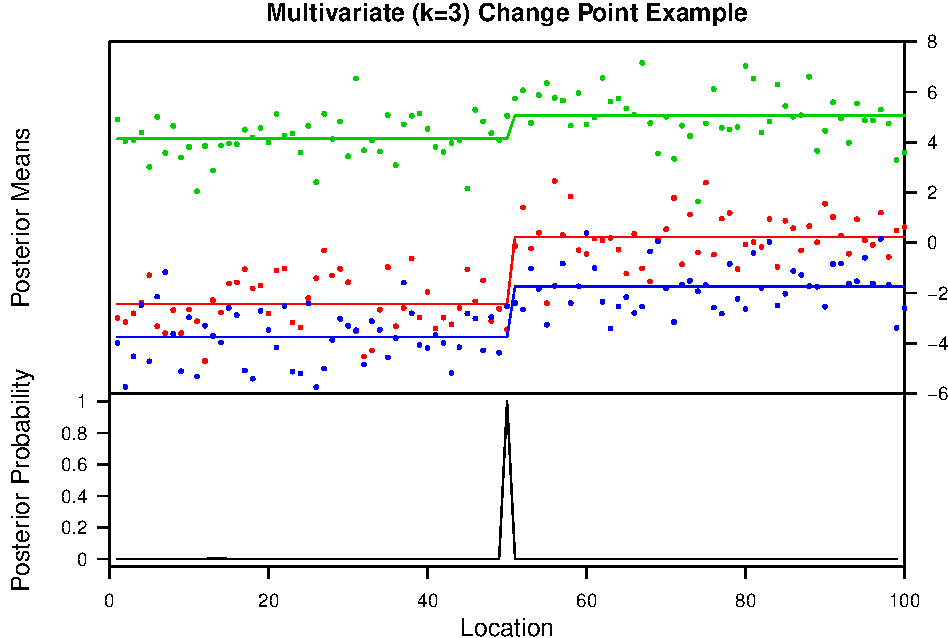
\includegraphics{rentersAndOwners_files/figure-latex/unnamed-chunk-7-1.pdf}

\begin{Shaded}
\begin{Highlighting}[]
\KeywordTok{plot}\NormalTok{(bcp.2a, }\DataTypeTok{separated=}\OtherTok{TRUE}\NormalTok{, }\DataTypeTok{main=}\StringTok{"Multivariate (k=3) Change Point Example"}\NormalTok{)}
\end{Highlighting}
\end{Shaded}

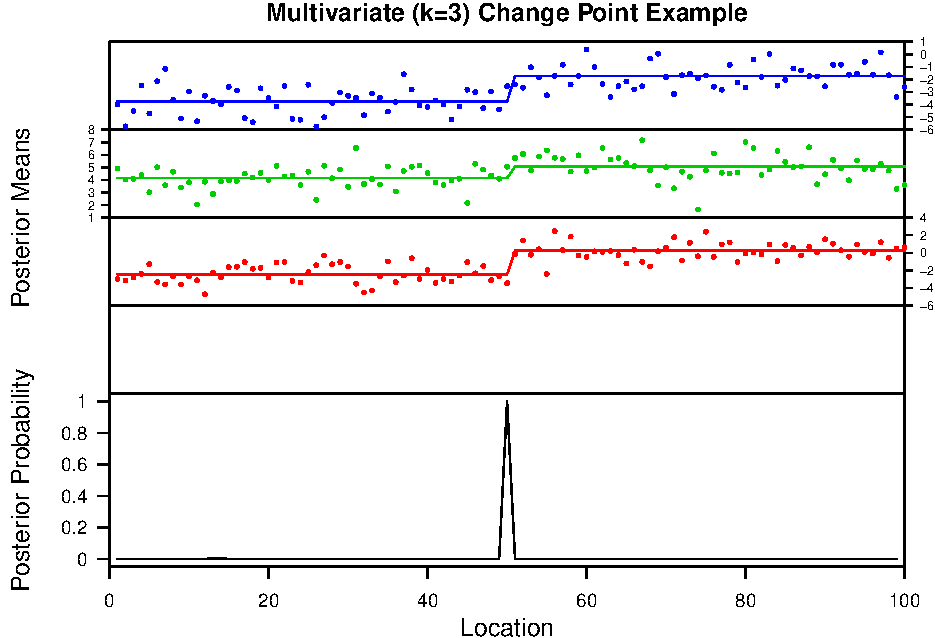
\includegraphics{rentersAndOwners_files/figure-latex/unnamed-chunk-7-2.pdf}

```


\end{document}
